\chapter{Cấu tạo mắt và sự lưu ảnh trên màng lưới}
\section{Lý thuyết trọng tâm}

\subsection{Cấu tạo quang học của mắt}
\begin{center}
	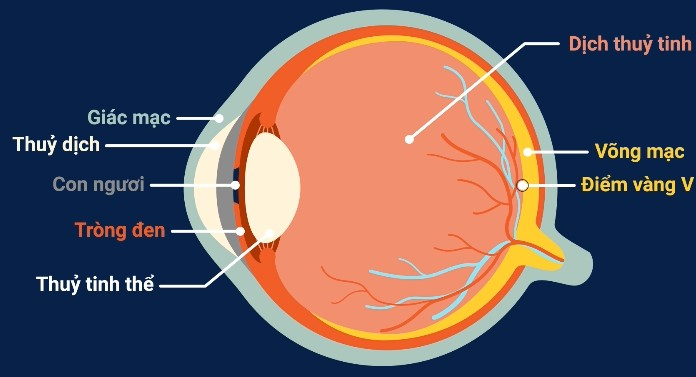
\includegraphics[scale=0.65]{../figs/VN11-PH-40-L-028-1-h32.jpg}
\end{center}
Từ ngoài vào trong, mắt có các bộ phận cơ bản sau:

\begin{description}
	\item [Giác mạc] là lớp màng cứng trong suốt, làm khúc xạ các tia sáng vào mắt.
	\item [Thủy dịch] là chất lỏng trong suốt. 
	\item [Tròng đen] là màn chắn, ở giữa có lỗ trống gọi là con ngươi, để điều chỉnh chùm ánh sáng đi vào trong mắt. 
	\item [Thể thủy tinh] là khối chất đặc trong suốt có hình dạng thấu kính hai mặt lồi, hay thấu kính hội tụ.
	\item [Dịch thủy tinh] là chất lỏng dạng keo loãng, lấp đầy nhãn cầu.
	\item [Màng lưới] hay còn gọi là võng mạc, đóng vai trò như một màn ảnh, mà tại đó có các tế bào nhạy sáng nằm ở đầu các dây thần kinh thị giác.
	\begin{itemize}
	\item Trên màng lưới có một chỗ rất nhỏ màu vàng, là nơi cảm nhận ánh sáng nhạy nhất, được gọi là \textbf{điểm vàng V}.
	
	\item Dưới điểm vàng V một chút là \textbf{điểm mù M} hoàn toàn không cảm nhận được ánh sáng.
    \end{itemize}
\end{description}

Trong quang học, mắt được biểu diễn bởi sơ đồ tượng trưng như hình và gọi là mô hình mắt thu gọn. 
\begin{center}
	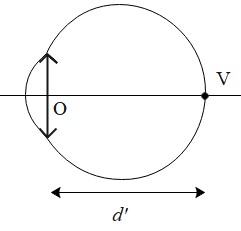
\includegraphics[scale=0.8]{../figs/VN11-PH-40-L-028-1-h33.jpg}
\end{center}
Trong mô hình đó, hệ quang học phức tạp của mắt được coi tương đương với một thấu kính hội tụ và gọi là thấu kính mắt.

Tiêu cự của thấu kính mắt thường gọi tắt là tiêu cự của mắt và cũng được kí hiệu là $f$.

Tổng quát, mắt hoạt động như một máy ảnh, trong đó: 
\begin{itemize}
	\item Thấu kính mắt có vai trò như vật kính;
	\item Màng lưới có vai trò như phim.
\end{itemize}

\subsection{Hiện tượng lưu ảnh của mắt}
Tác động của ánh sáng lên màng lưới còn tồn tại khoảng $\frac{1}{10}$ giây sau khi ánh sáng tắt. Đó là hiện tượng \textit{lưu ảnh của mắt.}

Nhờ hiện tượng này mà mắt nhìn thấy các ảnh trên màn hình chiếu phim, màn hình ti vi,... chuyển động. 

\section{Bài tập}
\begin{dang}{Cấu tạo của mắt}
\end{dang}
\viduii{1}{

Nhận xét nào sau đây là đúng?
\begin{mcq}
	\item Có thể coi hệ quang học phức tạp của mắt tương đương với một thấu kính phân kỳ.
	\item Nơi cảm nhận ánh sáng nhạy nhất, được gọi là điểm mù M.
	\item Điểm vàng V hoàn toàn không cảm nhận được ánh sáng.
	\item Thể thủy tinh là khối chất đặc trong suốt có hình dạng thấu kính hai mặt lồi, hay thấu kính hội tụ.
\end{mcq}}{
\begin{center}
	\textbf{Hướng dẫn giải:}
\end{center}

{ Câu A sai vì có thể coi hệ quang học phức tạp của mắt tương đương với một thấu kính hội tụ.
	
	Câu B sai vì nơi cảm nhận ánh sáng nhạy nhất, được gọi là điểm vàng V.
	
	Câu C sai vì điểm mù M mới nơi hoàn toàn không cảm nhận được ánh sáng.
	
\textbf{	Đáp án: D.}
}
}
\viduii{1}{
Kết luận nào sau đây là \textbf{không đúng} khi so sánh mắt và máy ảnh?
\begin{mcq}
	\item Thủy tinh thể có vai trò giống như vật kính. 
	\item Ảnh thu được trêm phim của máy ảnh và trên võng mạc của mắt có tính chất giống nhau, đều là ảnh thật.
	\item Ảnh thu được trêm phim của máy ảnh và trên võng mạc của mắt có tính chất khác nhau, đều là ảnh ảo.
	\item Màng lưới có vai trò giống như phim.
\end{mcq}}{
\begin{center}
	\textbf{Hướng dẫn giải:}
\end{center}

{ Câu C không đúng vì ảnh thu được trêm phim của máy ảnh và trên võng mạc của mắt có tính chất giống nhau, đều là ảnh thật. 
	
\textbf{	Đáp án: C.}
}
}
\begin{dang}{Sự lưu ảnh của mắt}
\end{dang}
\vidu{1}{
Khi chiếu phim, để người xem có cảm giác quá trình đang xem diễn ra liên tục, thì các cảnh quay thường cách nhau một khoảng thời gian là
\begin{mcq}
	\item $\dfrac{1}{10}$ giây 
	\item 10 giây
	\item 1 giây
	\item $\dfrac{1}{2}$ giây
\end{mcq}}{
\begin{center}
	\textbf{Hướng dẫn giải:}

\end{center}
{ Tác động của ánh sáng lên màng lưới còn tồn tại khoảng $\dfrac{1}{10}$ giây sau khi ánh sáng tắt.
	
\textbf{Đáp án: C.}
}

}
